\documentclass[letterpaper, 12pt]{article}


\usepackage{parskip,xspace}
\usepackage{amsmath,amsthm,amsfonts,amssymb}
\usepackage{mathrsfs} 
\usepackage{caption}
\usepackage{xcolor} 
\usepackage{geometry}
\usepackage{fancyhdr}
\usepackage{rotating}
\usepackage{multirow}
\usepackage{makecell}
\usepackage{ltxtable}
\usepackage{hyperref}
\usepackage{graphicx}
\usepackage{subfigure}
\usepackage{bm}
\usepackage[]{statrep}
\usepackage{enumerate}
\usepackage{subfigure}
\usepackage[toc,page]{appendix}

\graphicspath{{eps/}}


\newcommand{\ba}{$$\begin{aligned}}
\newcommand{\ea}{\end{aligned}$$}
\newcommand{\dx}{\mathrm{d}x}
\newcommand{\lma}{\left(\begin{matrix}}
\newcommand{\rma}{\end{matrix}\right)}




\pagestyle{fancy}
\lhead{Peng Shao 14221765}
\chead{}
\rhead{\bfseries STAT 8320 Spring 2015 Assignment 6}
\renewcommand{\headrulewidth}{0.4 pt}
\setlength{\parindent}{2em}

\begin{document}
\title{STAT 8320 Spring 2015 Assignment 6}
\author{Peng Shao 14221765}
\maketitle
\indent




$\blacktriangleright$ \textbf{1.\quad Solution.} 
(a). Because PCA is not invariant with respect to changes in scale, that is, the variable which is measured under larger scale will have larger variance, then produce a large eigenvalue when performing singular value decomposition. So standardization avoids the problems of having one variable with large variance unduly influencing the determination of factor loadings, and the correlation matrix is the covariance matrix of standardized variable.

(b). Before PCA, we should investigate the data roughly, and we find that there may be an outlier which have the total score less than 6000. We have no idea why cause this abnormality, but we should take it out of the following analysis because the PCA is very sensitive to outliers. Then we do a PCA based on the 10 single scores.

\begin{figure}[htbp]
\centering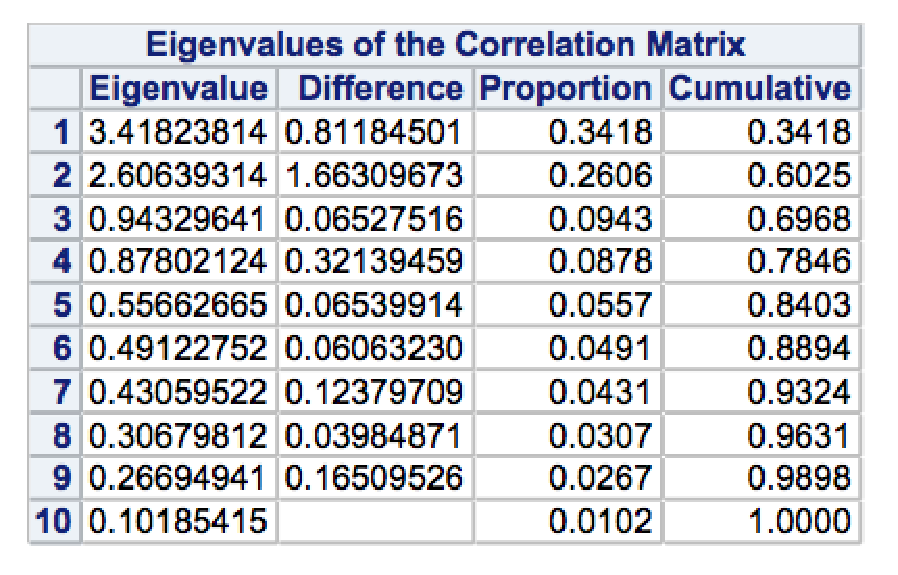
\includegraphics[width=3.5in]{7-1.eps}
\caption{Principal Component Proportion}\label{1}
\end{figure}

From Figure \ref{1}, the first 2 PCs have accounted for 60.25\% variability of the total.


(c).
Because the first 2 PCs account for more than 50\% variability of the data, and the only these 2 PCs have the eigenvalues more than 1.

(d). 
\begin{figure}[htbp]
\centering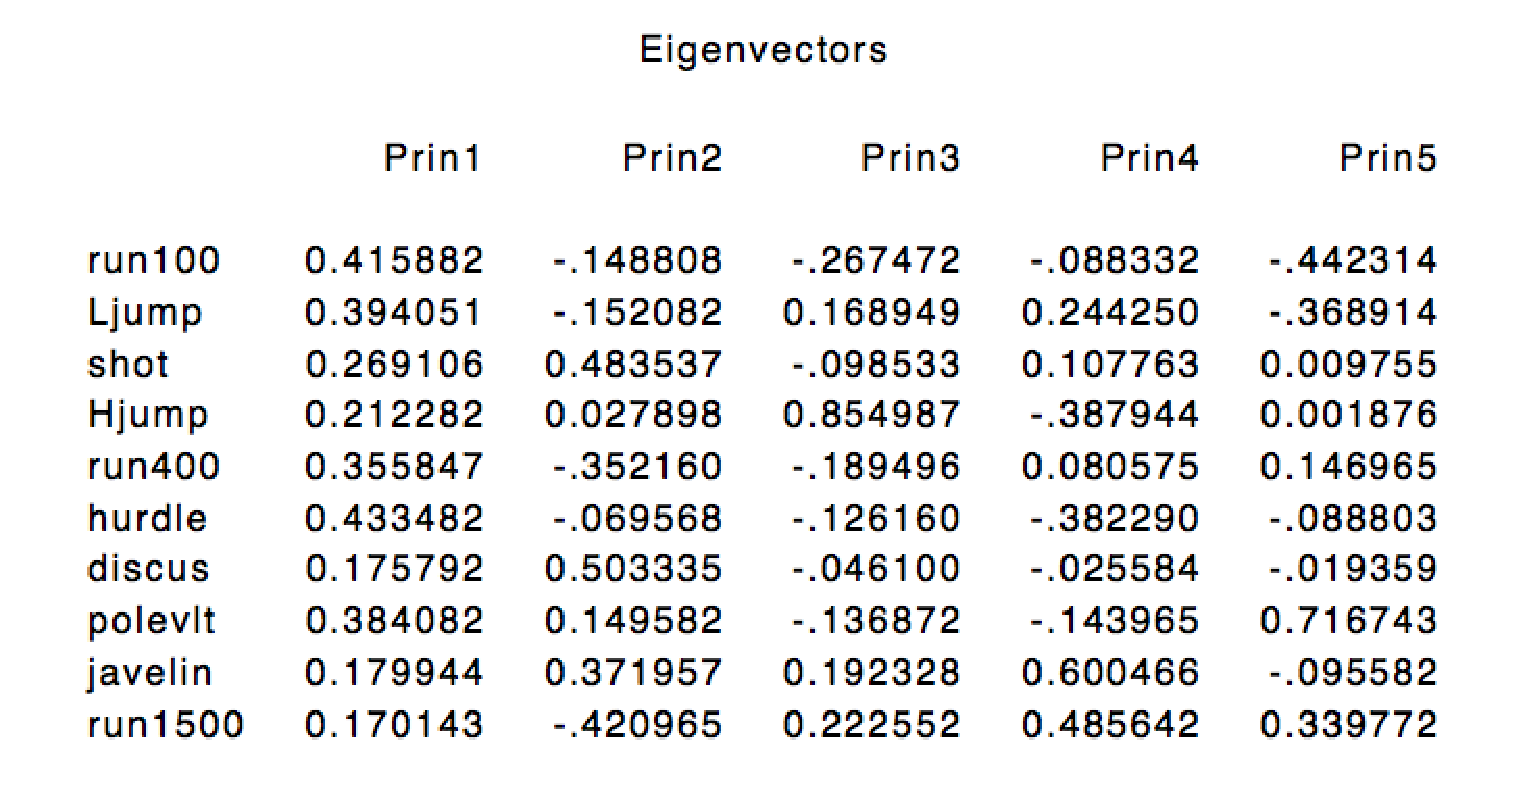
\includegraphics[width=5in]{7-2.eps}
\caption{First 5 Principal Components}\label{2}
\end{figure}
According to the part of PC table (Figure \ref{2}), the first principal component may be a kind of overall means of all scores, not exactly equal to the average because of some slightly different weights; and the second principal component may be the comparison between the scores of running add long jump and those of throwing add pole vault. 


(e). \begin{figure}[htbp]
\centering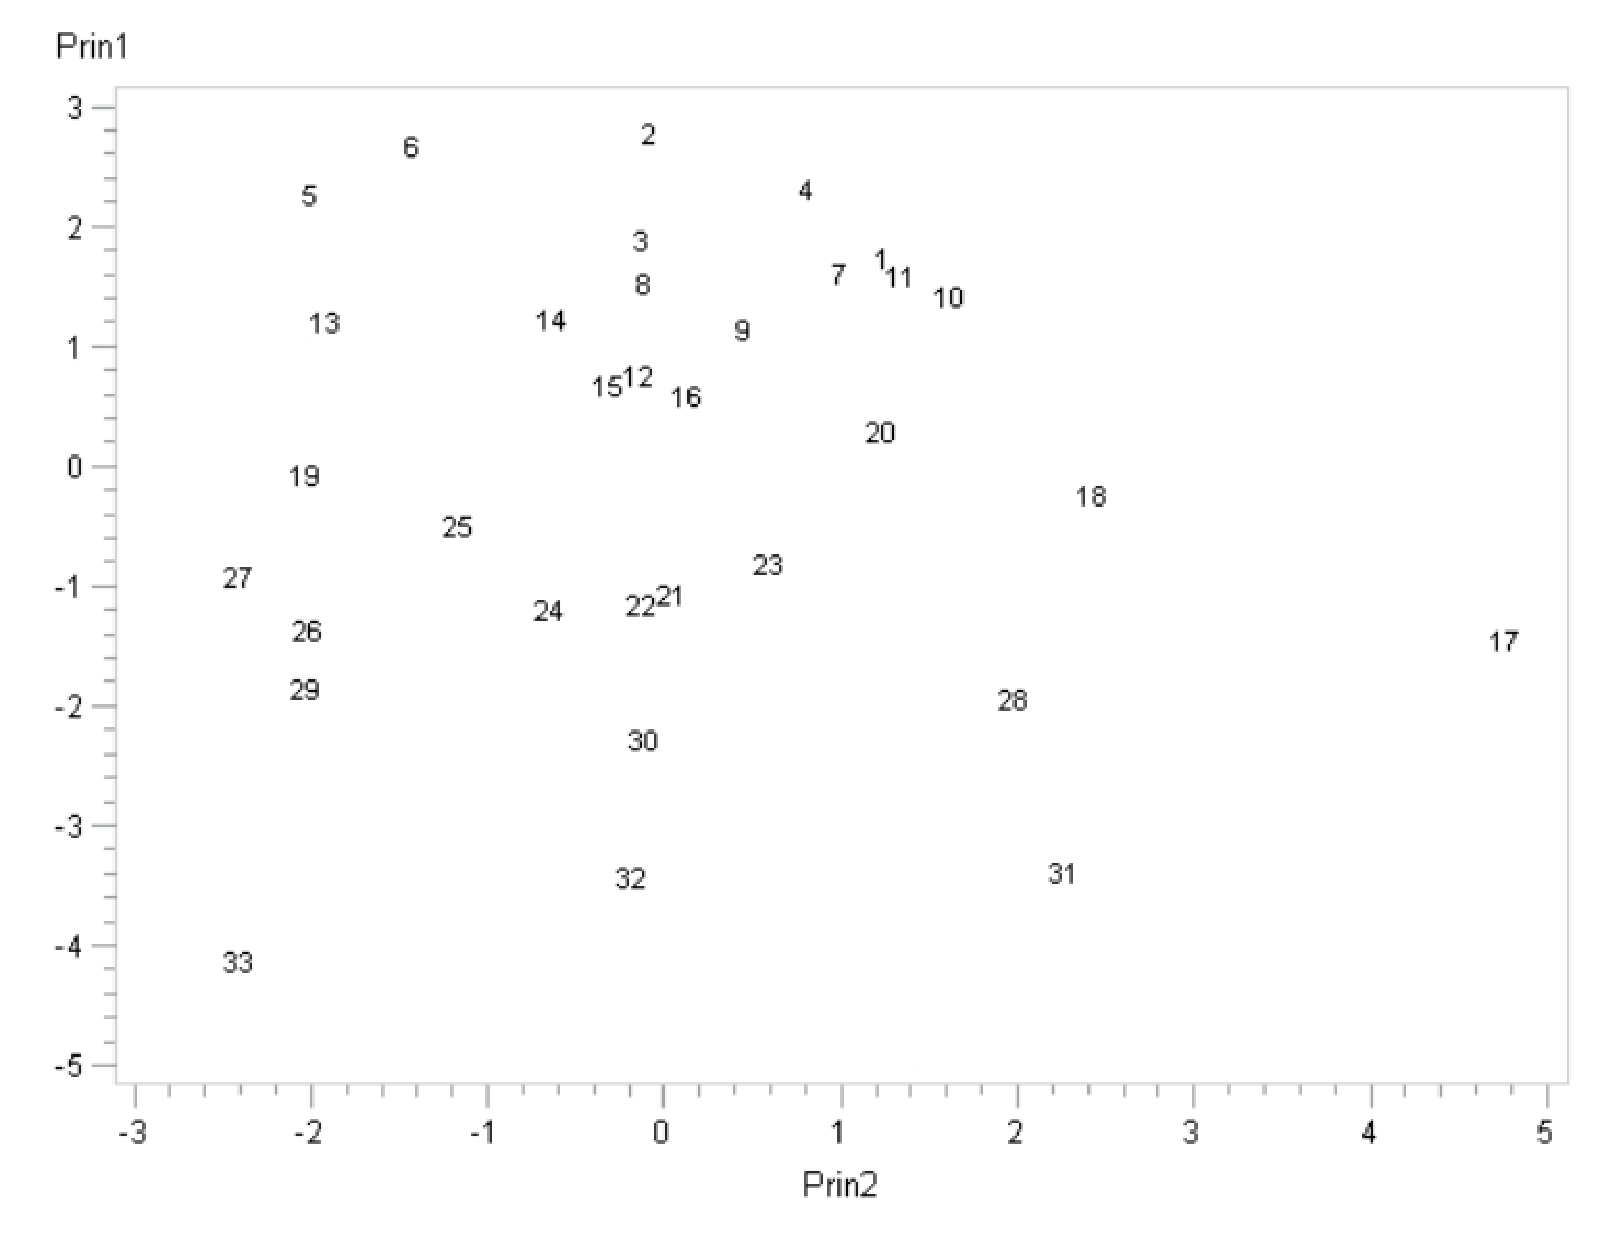
\includegraphics[width=5in]{7-3.eps}
\caption{1st PC v.s. 2nd PC}\label{3}
\end{figure}

From the scatter plot Figure \ref{3}, the data points have already been labeled as the their rank. So we can see that most high rank athletes (here higher rank means higher total score but smaller value of the rank) have comparably high 1st PC score. However, it is hard to see that whether there is any pattern of 2nd PC score relative to the ranks of athletes. 

Hence, to make the relationship between PC scores and the ranks (or the total scores) more clearly, we can plot the total score versus two PC scores respectively(Figure \ref{4} and Figure \ref{5}). From Figure \ref{4}, we can see that the 1st PC score has positive relationship with total score indeed, and we also believe that there should be no significant relationship between 2nd PC score and total score.
\begin{figure}[htbp]
\begin{minipage}[t]{0.5\linewidth}
\centering
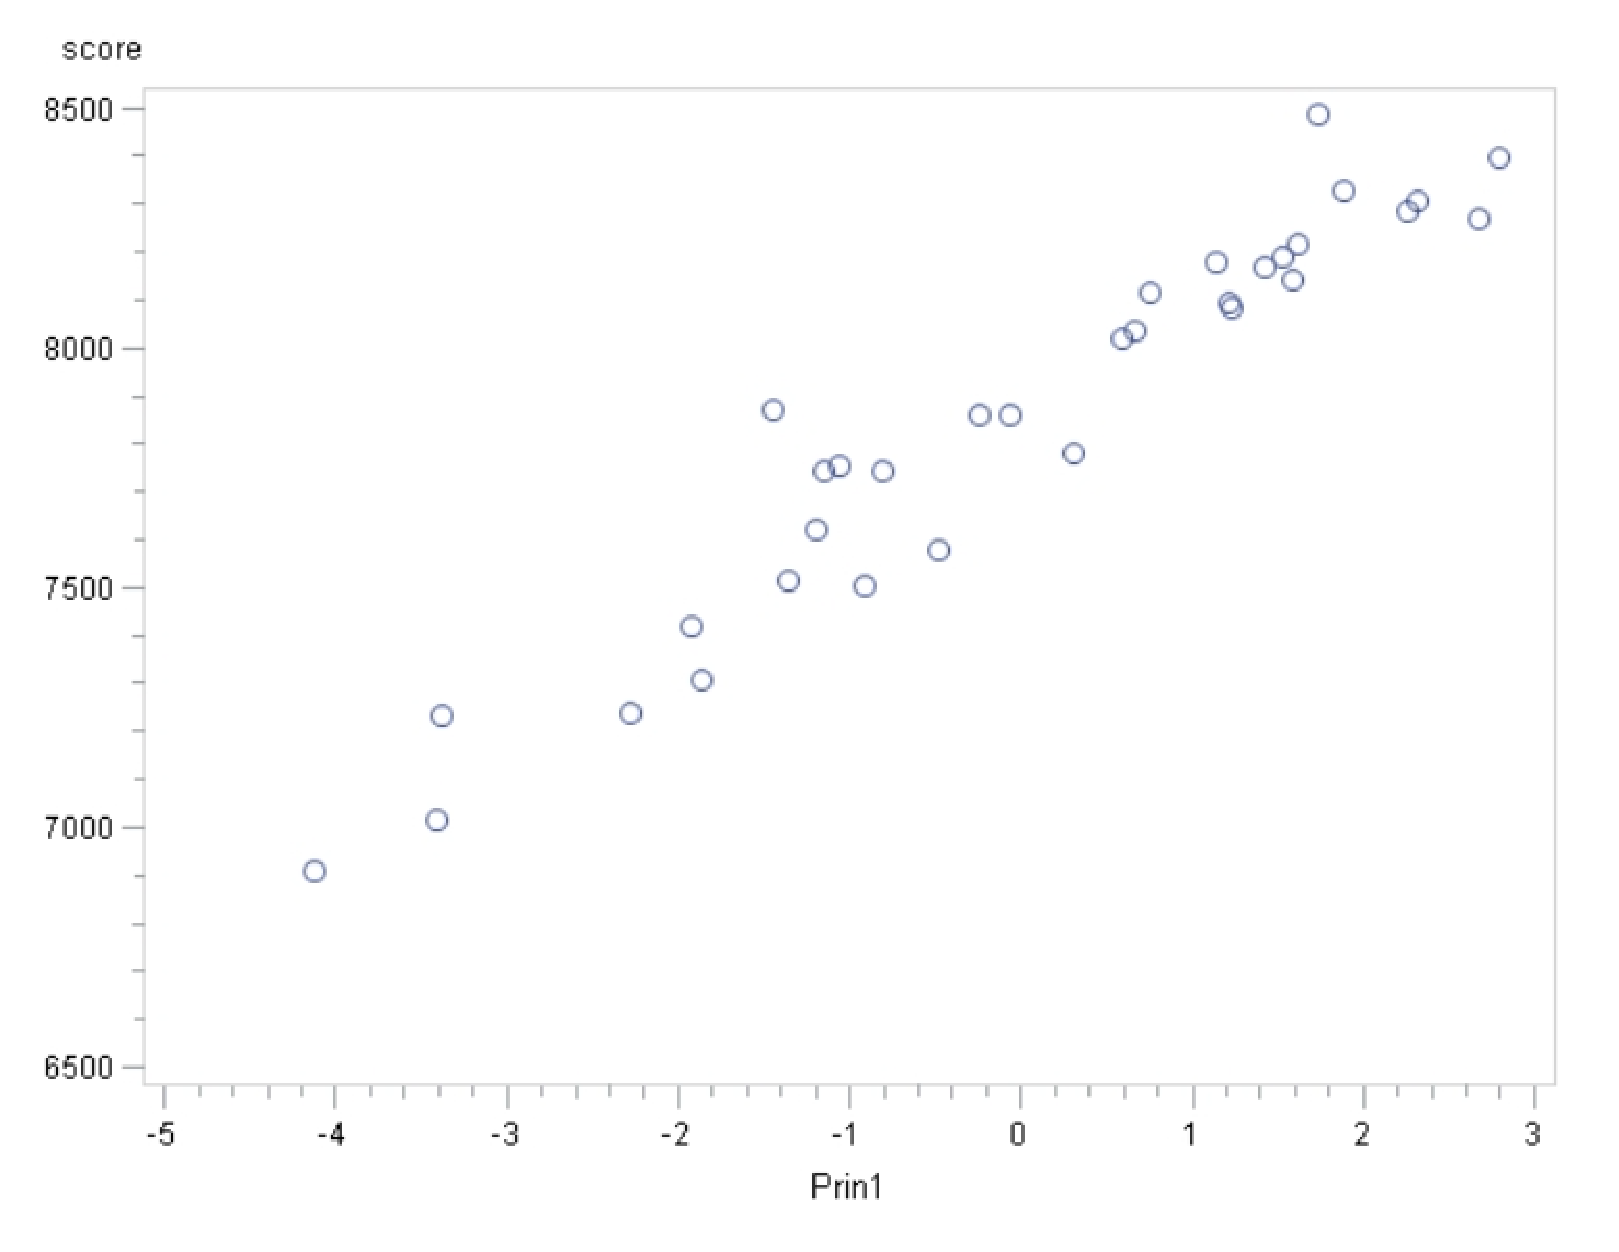
\includegraphics[width=3in]{7-4.eps}
\caption{Total Score v.s. 1st PC}\label{4}
\end{minipage}
\begin{minipage}[t]{0.5\linewidth}
\centering
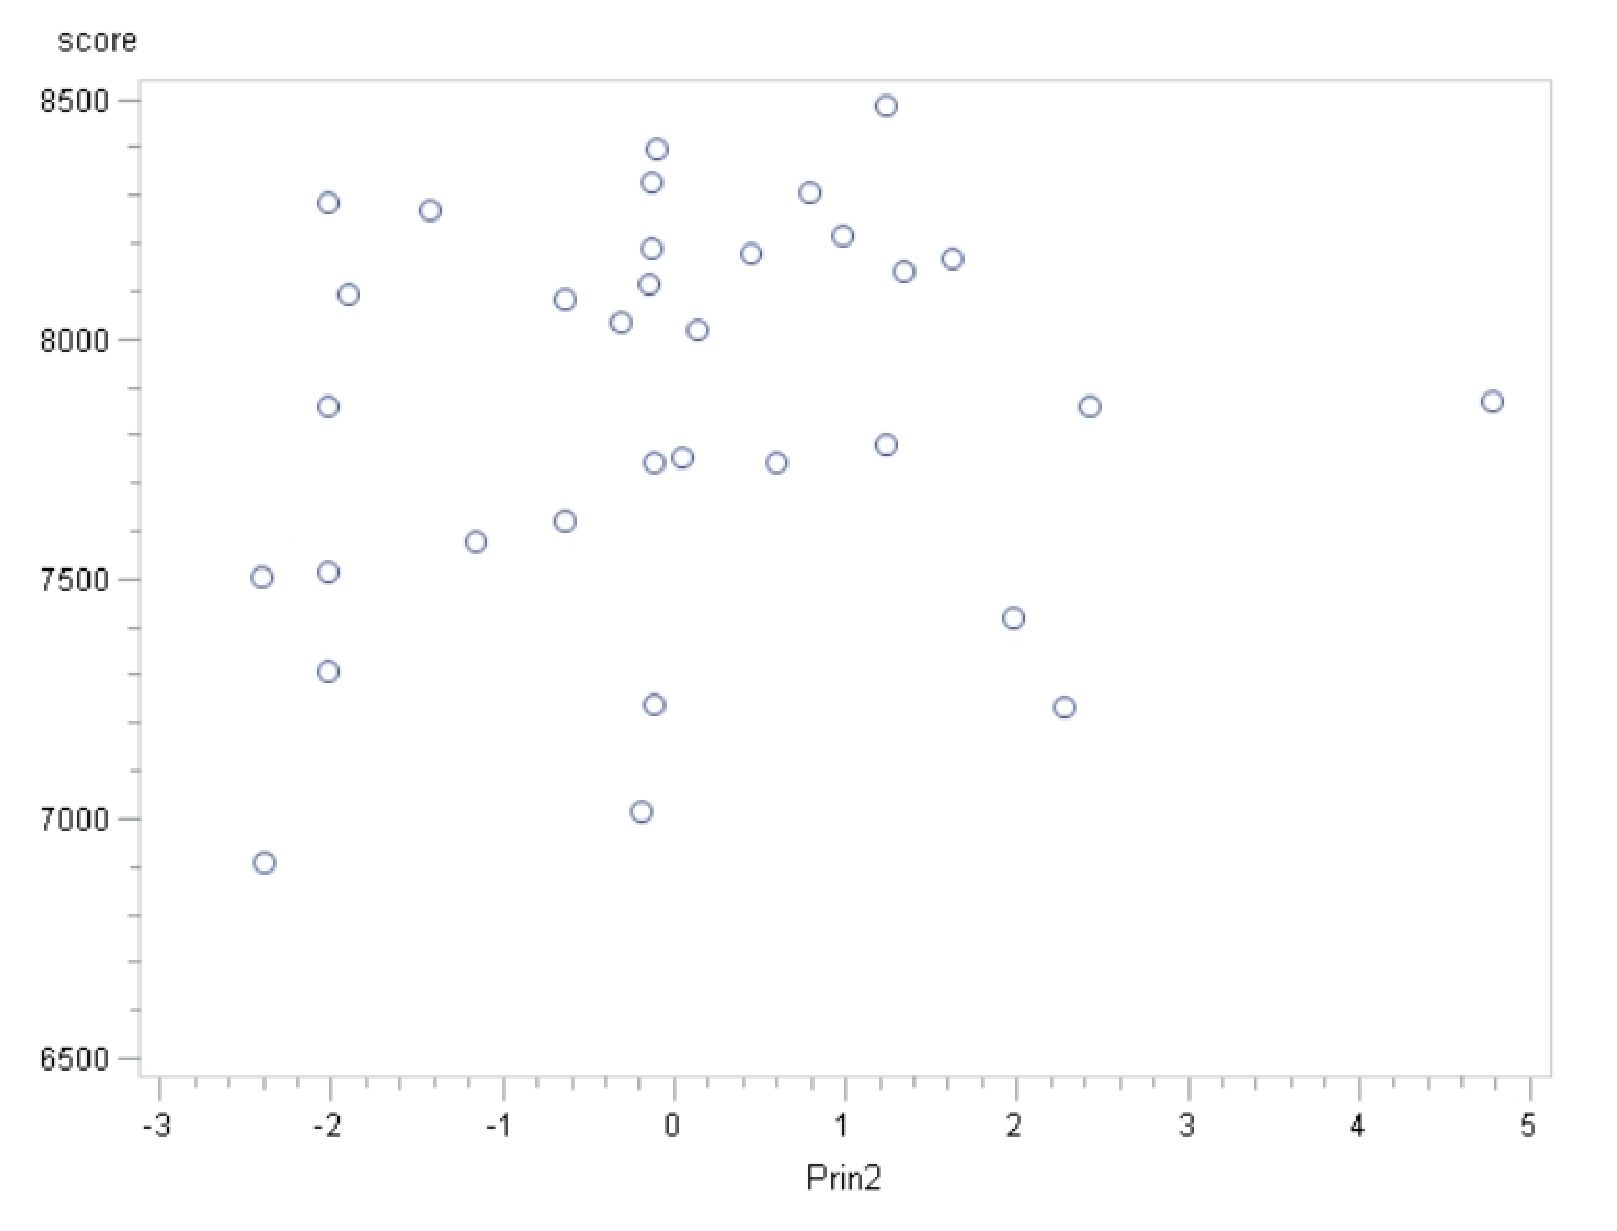
\includegraphics[width=3in]{7-5.eps}
\caption{Total Score v.s. 2nd PC}\label{5}
\end{minipage}
\end{figure}


(f). \begin{figure}[htbp]
\centering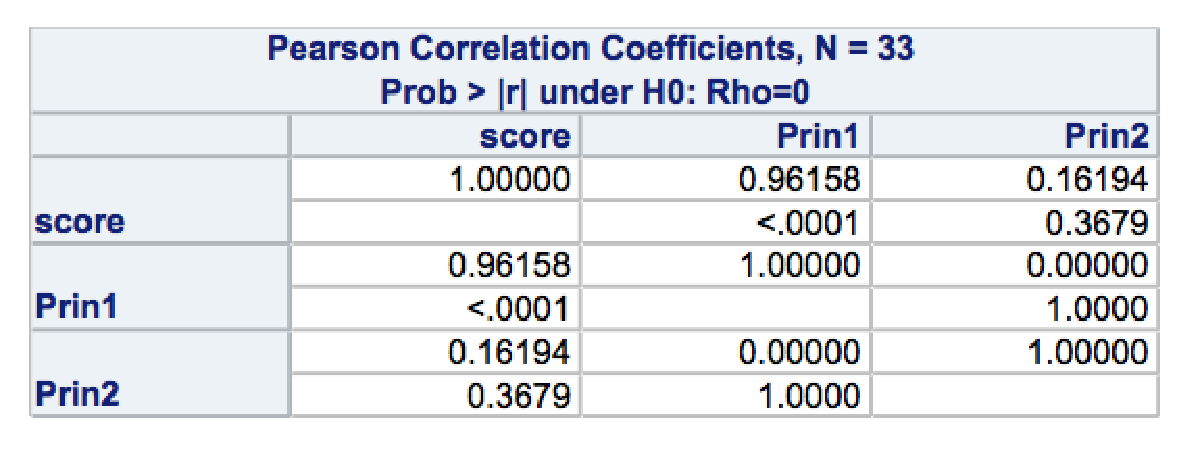
\includegraphics[width=4in]{77.eps}
\caption{Correlation Matrix among PCs}
\end{figure}

To compute the Pearson correlation coefficients among the total score, 1st PC score and 2nd PC score. The correlation coefficient between total score and 1st PC score is 0.96158 while that between total score and 2nd PC score is only 0.16194. This is in accordance with the result of last part. Thus, we may guess that the total score should be measured in a way like 1st PC, i.e., a kind of overall mean, not some comparisons.




$\blacktriangleright$ \textbf{2.\quad Solution.} 
(a). Because $X_i$ are standardized random variables(zero mean and one standard deviation), then the covariance of $X_i$ is exactly the correlation of $X_i$. So
\ba
corr(X_i,X_k)&=cov(X_i,X_k)=cov(a_iF+e_i,a_kF+e_K)\\
&=a_ia_kvar(F)+a_icov(F,e_k)+a_kcov(e_i,F)+cov(e_i,e_k)=a_ia_k\\
corr(X_j,X_k)&=cov(X_j,X_k)=cov(a_jF+e_j,a_kF+e_K)\\
&=a_ja_kvar(F)+a_jcov(F,e_k)+a_kcov(e_j,F)+cov(e_j,e_k)=a_ja_k\\
\ea
where $i,j,k$ are mutually different. Thus the ratio of pair of rows $(i,j)$ is always
$$
\frac{corr(X_i,X_k)}{corr(X_j,X_k)}=\frac{a_i}{a_j}
$$
for all $k\not=i,j$.


(b). 
$$
corr(\bm{X})=\lma a_1\\a_2\\a_3\\a_4\\a_5\\a_6\rma\lma a_1&a_2&a_3&a_4&a_5&a_6\rma+var(\bm{e})
$$

(c). 
$$
\bm{X}=\bm{a}F+\bm{e}
$$
where 
\begin{itemize}
\item $\bm{X}=\lma X_1&X_2&\cdots&X_6\rma'\sim \text{N}(\bm{0},corr(\bm{X}))$
\item $F\sim\text{N}(0,1)$
\item $\bm{a}=\lma a_1&a_2&\cdots&a_6\rma'$
\item $\bm{e}=\lma e_1&e_2&\cdots&e_6\rma'\sim \text{N}(\bm{0},\bm{\Psi})$
\item $F$ and $\bm{e}$ are independent.
\end{itemize}


(d). For my perspective, only one factor should be included. Because
\begin{enumerate}
\item only the eigenvalue of the 1st factor is larger than 1, no matter how many factor we include in the analysis, and the proportion of variability accounted by the 1st factor is at least 100\%.
\item to test the hypothesis
$$
H_0:\text{ 1 Factor is sufficient}
$$
the P-value is 0.9805, so we cannot reject the null hypothesis, that is, more factors are not necessary.
\item the AIC and BIC of one factor are lower than those of two factors.
\end{enumerate}

(e). The result of "Factor Pattern" can give the information about factor loadings of different variable, i.e. the $a_i$ in the model in part (c). For example, the variable C has a loading of 0.95611(a very high loading) in Factor1, and the variable F has a loading of 0.87081(a moderately to high loading) in Factor1, and so on. All variables have a at least moderately to high loading in Factor1, and the loadings are not different so much.

In addition, we can know how much proportion of variance of each variable is accounted by the communality from the "Factor Pattern" output or "Final Communality" output. For example, 
$$
\text{Communality of C}=a_1^2=0.95611^2=0.9141
$$
which means 91.41\% variability of C comes from common factor and only 8.69\% variability come from specific factor.

(f). No. If the rotation is help, let $T$ become the rotation operator. Then we can have that
$$
F^*=TF
$$
where the $F^*$ is the factor after rotating. So the $F^*$ should also have the restriction of length equal to 1, i.e. $var(F^*)=1$. This implies that $T^2=1$, and so $T=\pm1$. So rotation cannot change the value of loadings except the sign. Thus, there is no need to perform a rotation.


(g). Because in part (e), the loadings of different variable are not exactly same, so the ratio of any two loadings are you 1, as part (a). states. and from the part (d), we only include one factor, so the correlation coefficient directly determined by the loadings. Then the correlation coefficients should not be same. The test result is not so consistent with the conclusion of part (d) and part (e). But we cannot say either of them is wrong, it is very probability that the test is not power enough to prove the alternative hypothesis of different correlation coefficient. 








$\blacktriangleright$ \textbf{3.\quad Solution.} 
(a). \begin{figure}[htbp]
\centering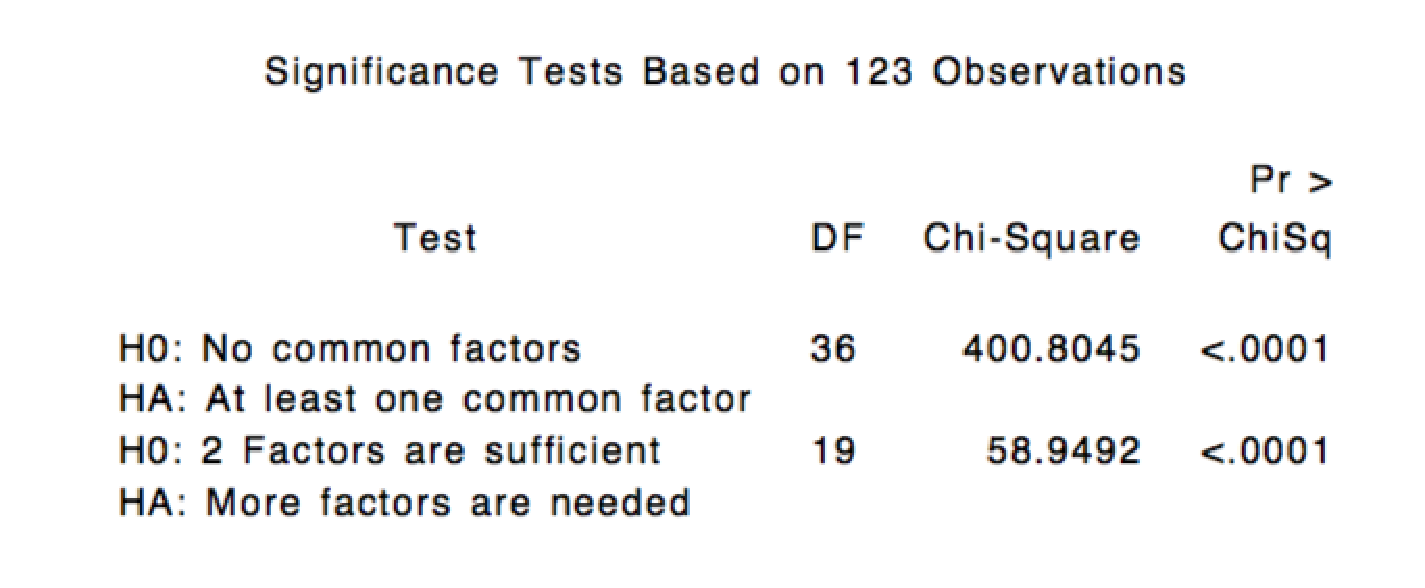
\includegraphics[width=4in]{7-6.eps}
\caption{Likelihood Tests}\label{6}
\end{figure}

No. From the second test in Figure \ref{6}, the P-value less than 0.0001 means we should reject the null hypothesis, that is, two factors is not sufficient.

(b). \begin{figure}[htbp]
\centering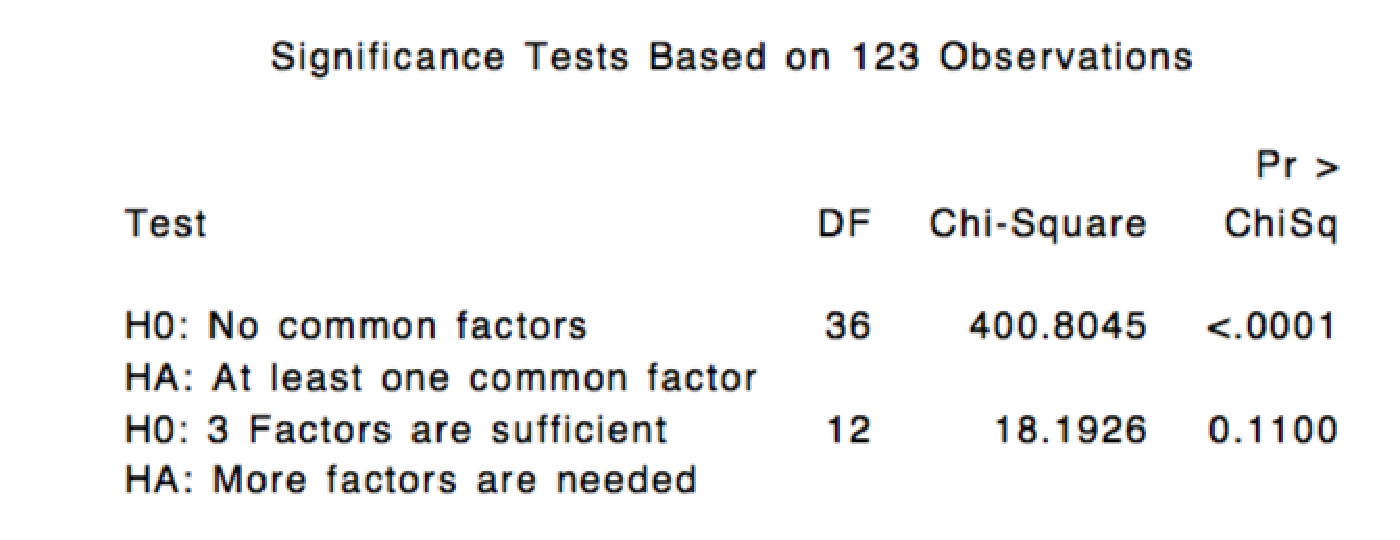
\includegraphics[width=4in]{7-7.eps}
\caption{Likelihood Tests}\label{7}
\end{figure}
Yes. From the second test in Figure \ref{7}, the P-value=0.1100 means we do not reject the null hypothesis, that is, 3 factors is sufficient.

\begin{figure}[htbp]
\centering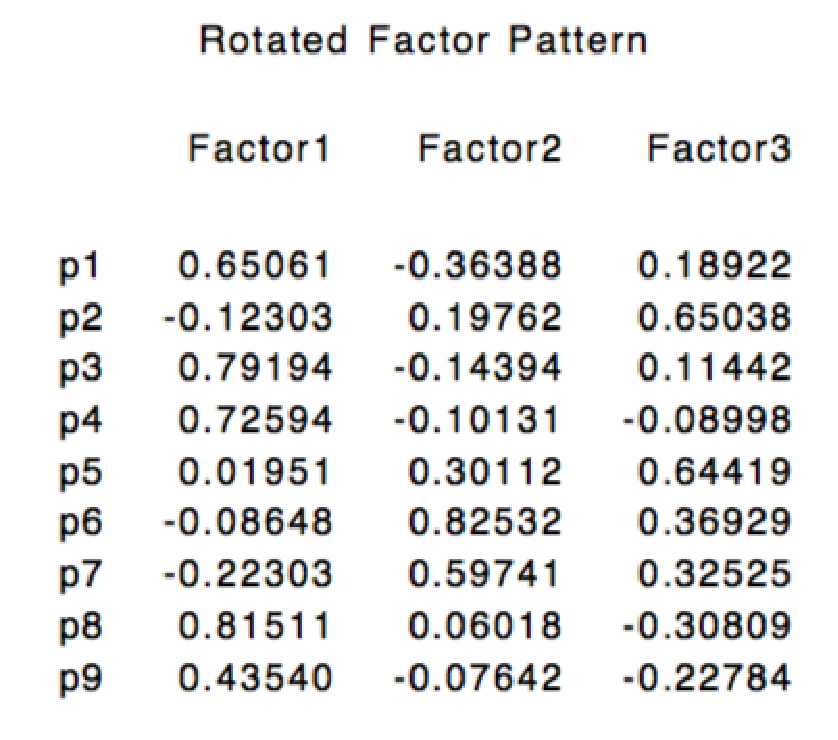
\includegraphics[width=3in]{7-8.eps}
\caption{Rotated Factors}\label{8}
\end{figure}
From the Figure \ref{8}, we can see that $p1,p3,p4,p8,p9$ have high loadings in factor 1, and all there statements have mentioned doctor. So maybe the factor 1 is a "doctor factor". $p6,p7$ have high loadings in factor 2, and all these statements is about themselves without some specific reasons. So maybe the factor 2 is a "subjective personal factor". $p2,p5$ have high loadings in factor 3, and all these statements is also about themselves but more reasonable. So maybe the factor 3 is a "objective personal factor".


(c). \begin{figure}[htbp]
\centering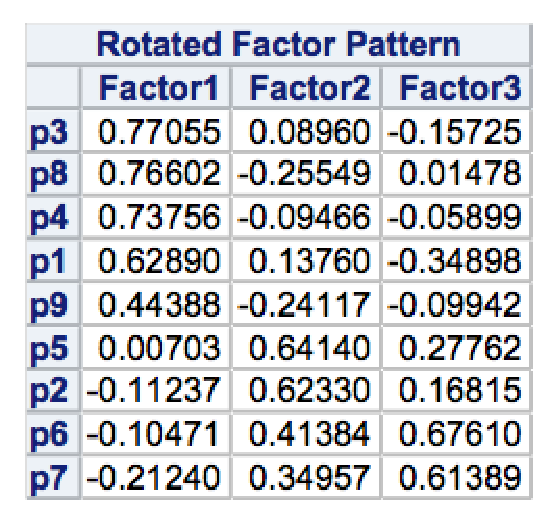
\includegraphics[width=2.5in]{7-9.eps}
\caption{Rotated Factors}\label{9}
\end{figure}
From the Figure \ref{9}, we can see that the factor pattern does not change too much between MLE and principle factor method; the clusters are still same: $\{p3,p8,p4,p1,p9\},\{p5,p2\},\{p6,p7\}$, only the loadings change slightly. But the interpretation becomes a little different. Because principle factor method uses the philosophy of PCA, so the factor interpretation may be like the interpretation of PCs. That is, factor 1 is the overall mean of $\{p3,p8,p4,p1,p9\}$, factor 2 is the overall mean of $\{p5,p2\}$ and factor 3 is the overall mean of $\{p6,p7\}$.


(d). \begin{figure}[htbp]
\centering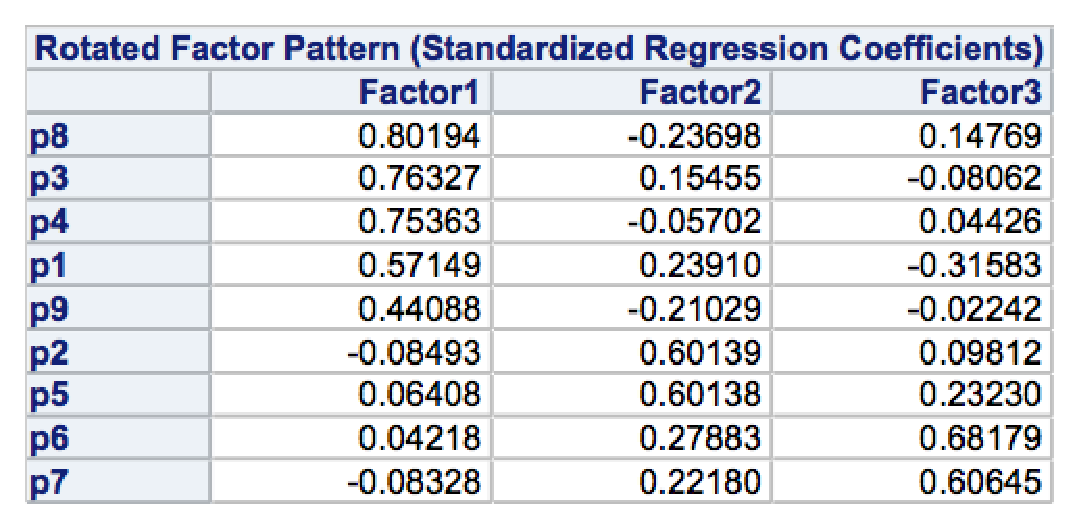
\includegraphics[width=4in]{7-10.eps}
\caption{Oblique Rotated Factors}\label{10}
\end{figure}
The overall result of principle factor method with oblique rotation is not so different from the result of other methods. It also only has some differences about factor loadings. The clusters and the interpretations of factors are same as the principle factor method with orthogonal rotation. However, for oblique rotation, we should also see the correlation between latent factors. In the problem the maximum correlation coefficient is 0.33129, which is not significant. So we can stop here. If the correlation between factors is significant, we can go on and perform a factor analysis to get the second order factor, which may contain more general information.

$\blacktriangleright$ \textbf{3.\quad Solution.} 
(a). The covariance matrices for spam and not-spam seem not same but we cannot perform most test because of the rank deficiency: the 41st attribute of not-spam is all 0.

Given the different correlation matrix, we should use the quadratic discriminant analysis. 





(b). Before all following analysis, we want to mention some index used in evaluating the performance of classifiers.
\begin{itemize}
\item \textbf{Precision}
$$
P=\frac{TP}{TP+FP}
$$
\item \textbf{Recall}
$$
R=\frac{TP}{TP+FN}
$$
\item \textbf{F-measure}
$$
F=\frac{2\cdot R\cdot P}{R+P}
$$
\item \textbf{Error Rate}
$$
ER=\frac{FP+FN}{P+N}
$$
\item \textbf{Missing Alarm}
$$
MA=1-R
$$
\item \textbf{False Alarm}\footnote{Here I choose false alarm instead of false positive rate because false alarm is more sensitive to the misclassification of negative case when positive cases are more rare. For example, we have 50 non-spam emails and 9 spam emails, and only one non-spam email is misclassified as spam, then the false positive rate is 2\% while false alarm is 10\%.}
$$
FA=1-P
$$
\end{itemize}

For the first three index, the larger the better; they give us the ability of prediction of the classifier; for the last three index, the lower the better; they give us the probabilities of misclassification of the classifier.
\begin{figure}[htbp]
\centering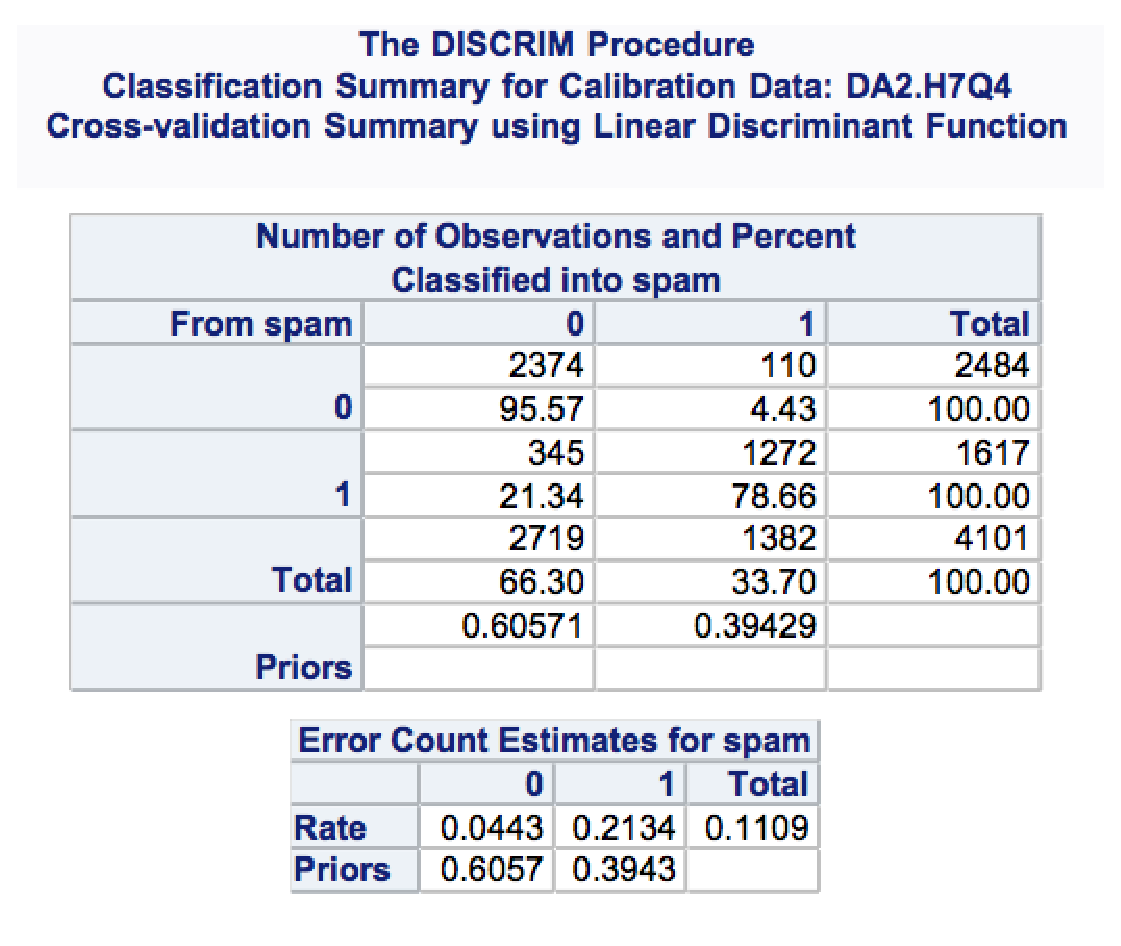
\includegraphics[width=3.5in]{7-100.eps}
\caption{Cross-validation for Linear Discriminant Funciton}\label{100}
\end{figure}

For cross-validation, we have
$$
TP=1272\quad FP=110\quad TN=2374\quad FN=345
$$
then we can compute that
\ba
&P=92.04\%\quad R=78.66\%\quad F=84.82\%\\
&ER=11.09\%\quad MA=21.34\%\quad FA=7.95\%
\ea
\begin{figure}[htbp]
\centering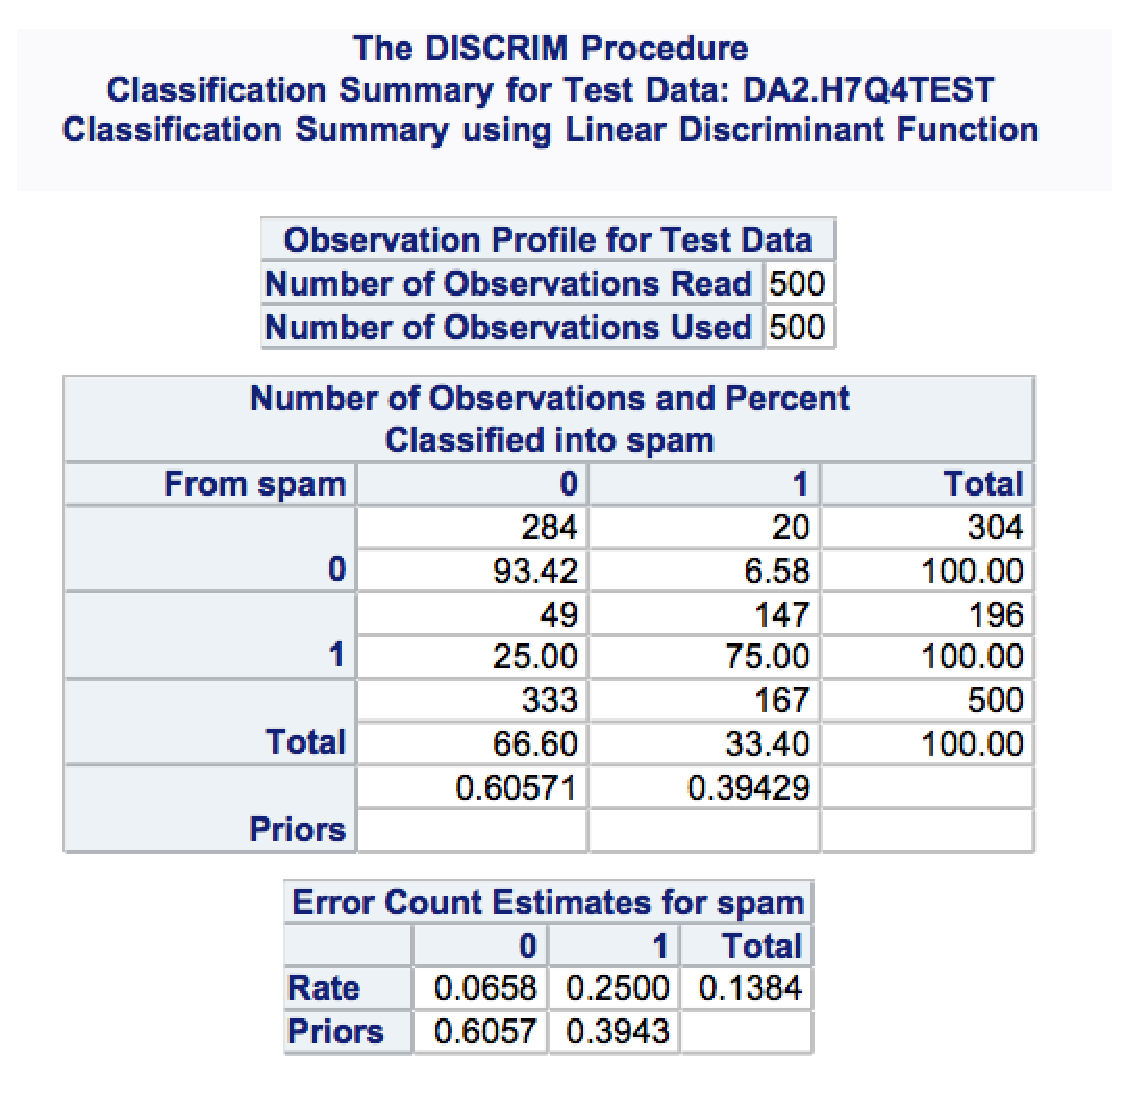
\includegraphics[width=3.5in]{7-11.eps}
\caption{Test for Linear Discriminant Funciton}\label{11}
\end{figure}

For test sample, we have
$$
TP=147\quad FP=20\quad TN=284\quad FN=49
$$
then we can compute that
\ba
&P=88.02\%\quad R=75\%\quad F=80.99\%\\
&ER=13.8\%\quad MA=25\%\quad FA=11.97605\%
\ea
It is very reasonable that the classifier has better performance on cross-validation than on testing sample, so the linear discriminant function is not bad.

(c).\begin{figure}[htbp]
\centering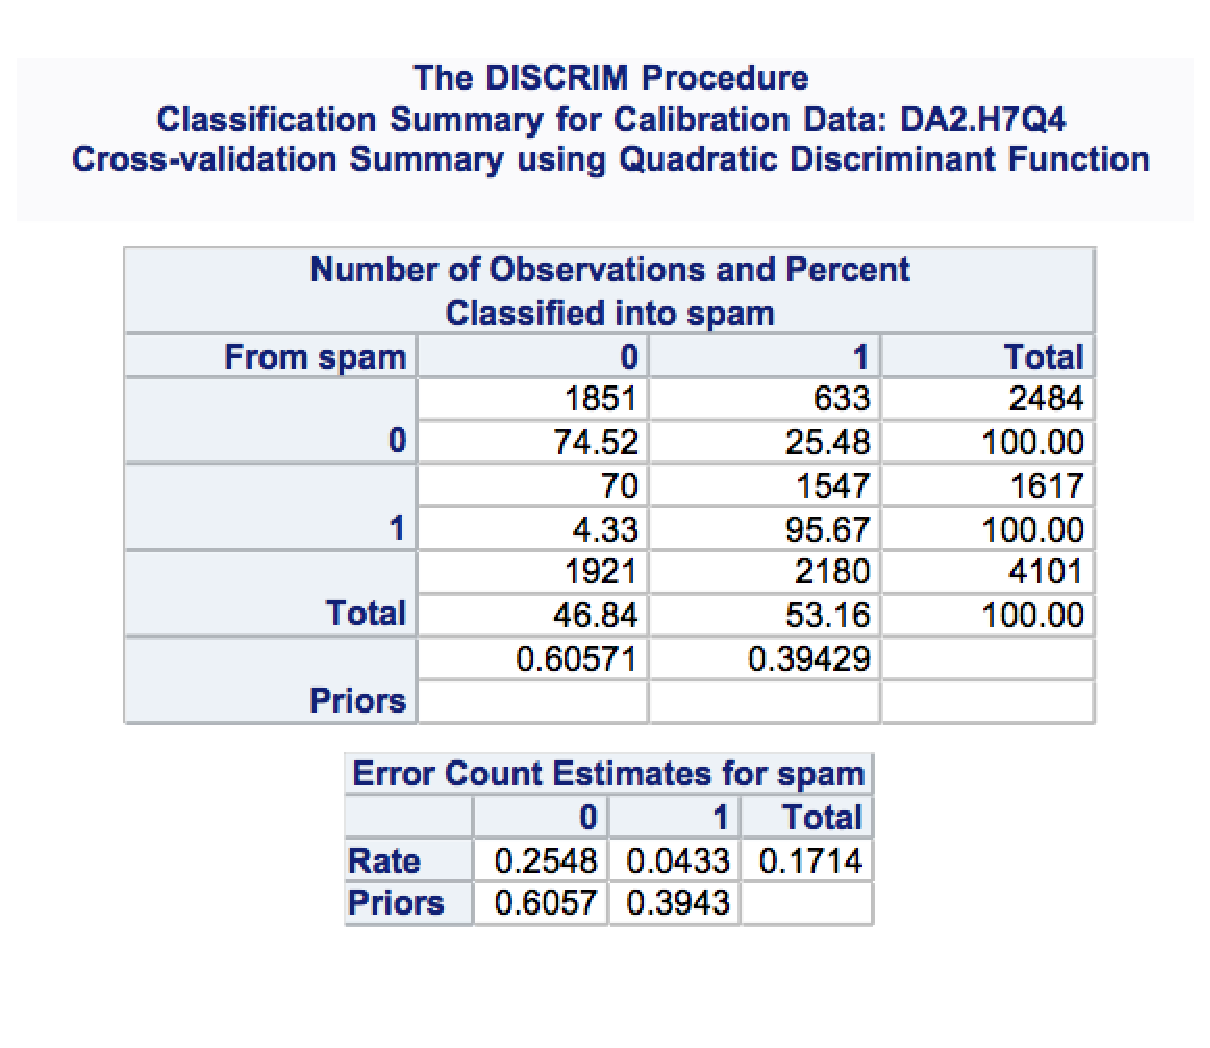
\includegraphics[width=3.5in]{7-12.eps}
\caption{Cross-validation for Quadratic Discriminant Funciton}\label{12}
\end{figure}

For cross-validation, we have
$$
TP=1547\quad FP=644\quad TN=1851\quad FN=70
$$
then we can compute that
\ba
&P=70.61\%\quad R=95.67\%\quad F=81.25\%\\
&ER=17.36\%\quad MA=4.33\%\quad FA=29.39\%
\ea
\begin{figure}[htbp]
\centering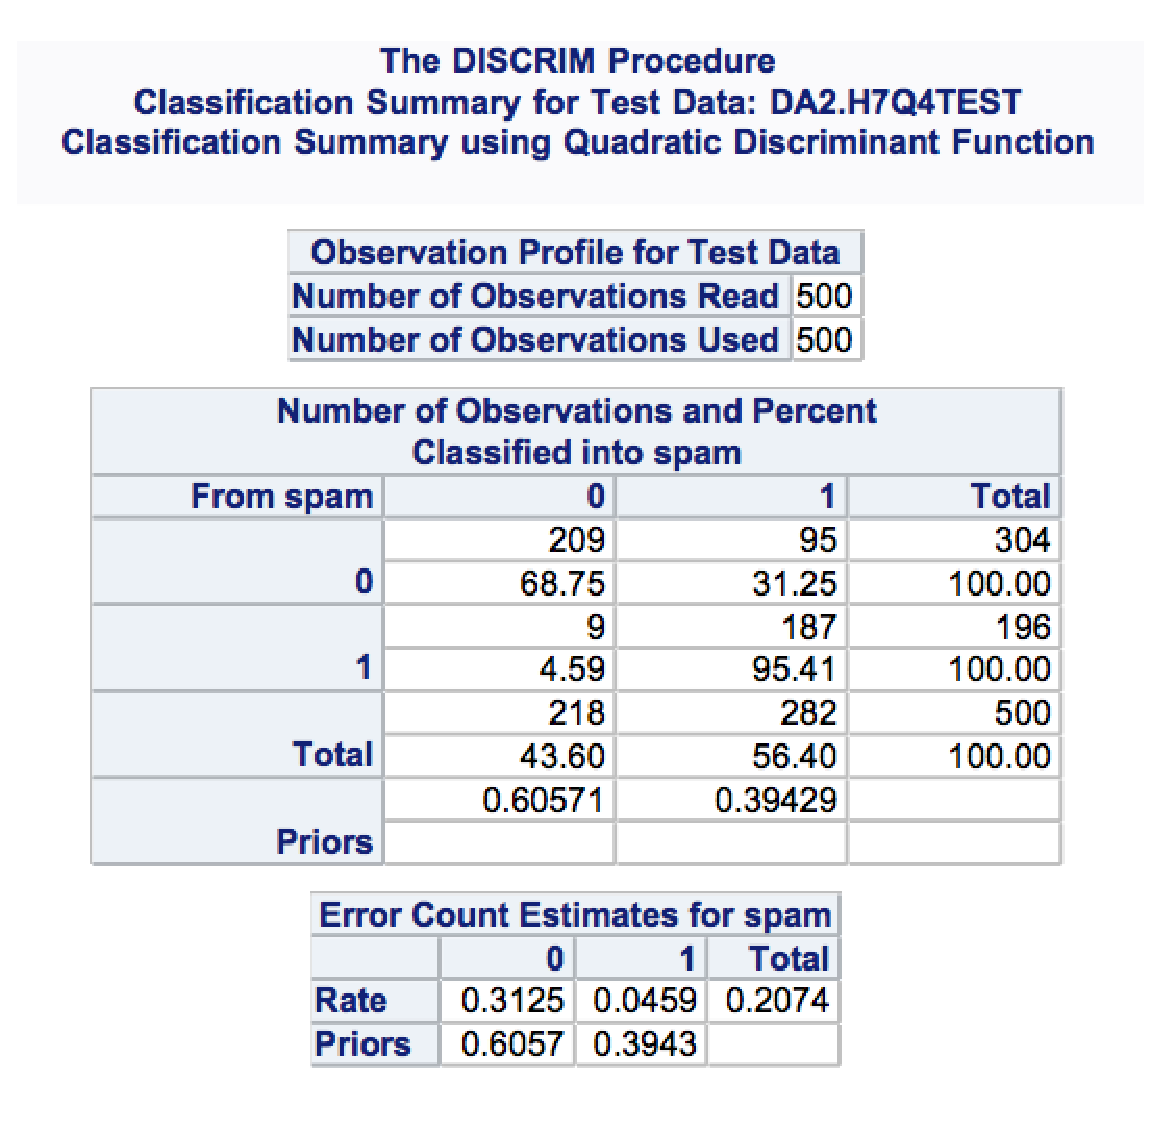
\includegraphics[width=3.5in]{7-13.eps}
\caption{Test for Quadratic Discriminant Funciton}\label{13}
\end{figure}

For test sample, we have
$$
TP=187\quad FP=95\quad TN=209\quad FN=9
$$
then we can compute that
\ba
&P=66.31\%\quad R=95.41\%\quad F=78.24\%\\
&ER=20.8\%\quad MA=4.59\%\quad FA=33.69\%
\ea

To compare the linear classifier, the quadratic classifier has higher recall and lower missing alarm, which indicates that it is excellent in detecting spam email; while in the meantime the false alarm become pretty large; it misclassify over 30 non-spam emails as spam emails, which could be very harmful.

(d).
\begin{figure}[htbp]
\centering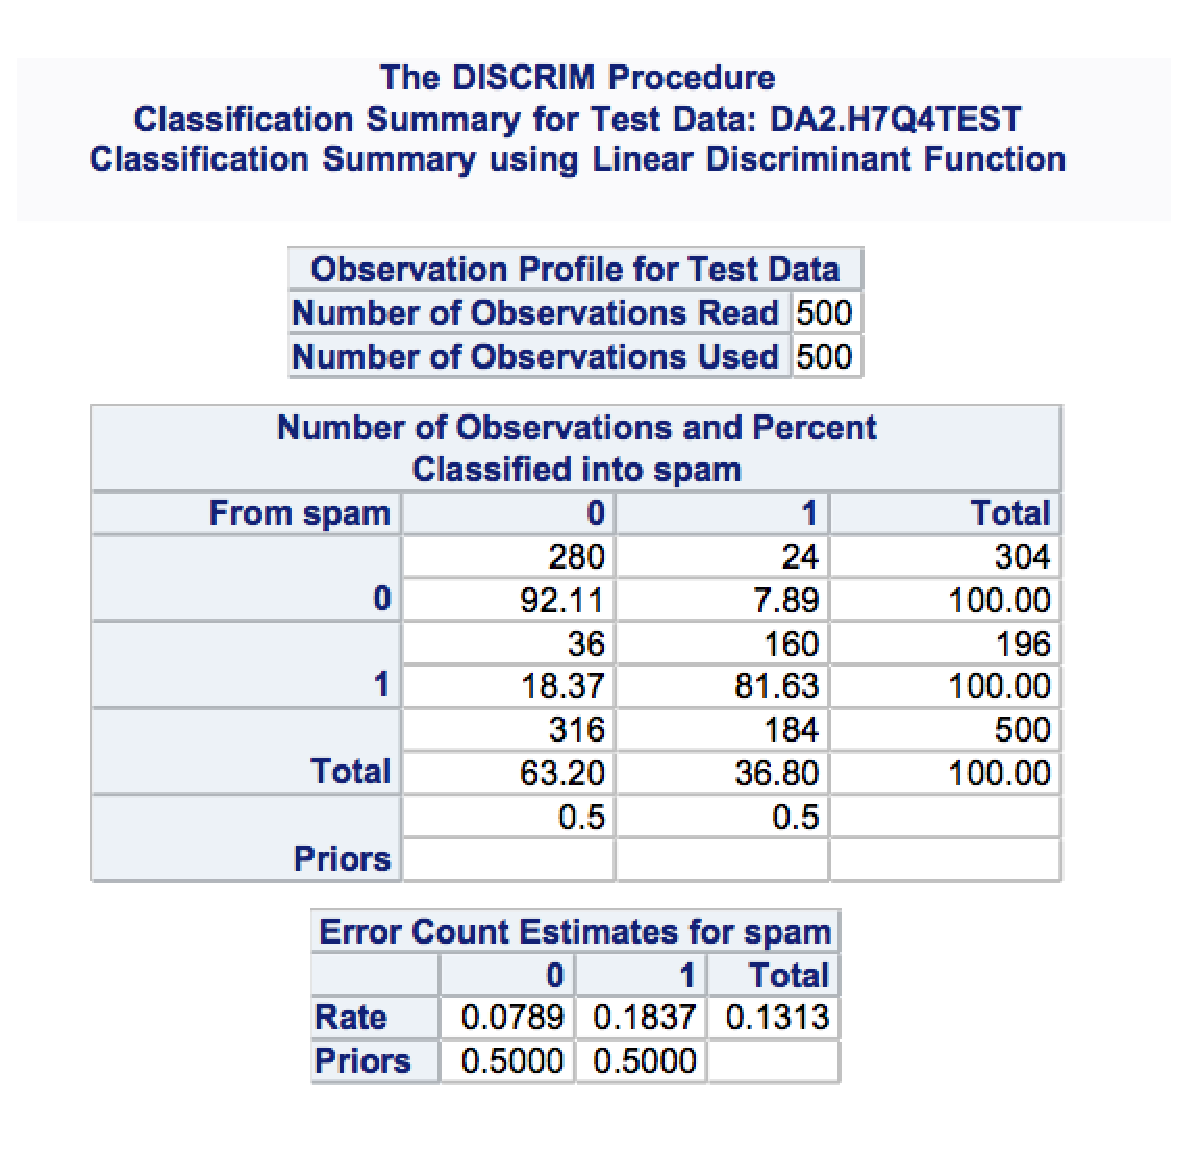
\includegraphics[width=3.5in]{7-14.eps}
\caption{Test for Step-selection Linear Discriminant Funciton}\label{14}
\end{figure}

For test sample, we have
$$
TP=184\quad FP=24\quad TN=280\quad FN=36
$$
then we can compute that
\ba
&P=88.46\%\quad R=83.64\%\quad F=85.98\%\\
&ER=11.45\%\quad MA=16.36\%\quad FA=11.54\%
\ea

Comparing to the two discriminant functions above, the linear discriminant function after stepwise selection has become a very good model. Because it has the highest $F$ score, the lowest error rate and lowest false alarm for test sample so far, which are what we are concerned about most. And its missing alarm is much less than the linear discriminant function with all attributes.


(e).\begin{table}
\centering
\begin{tabular}{|l|c|c|c|c|c|c|}
\hline
Model&P&R&F&ER\footnotemark[2]&MA&FA\\
\hline
2-Nearest Neighbors Classifier&99.44\%&99.79\%&99.61\%&8.46\%&0.21\%&0.56\%\\
\hline
3-Nearest Neighbors Classifier&94.34\%&93.11\%&93.72\%&5.32\%&6.89\%&5.66\%\\
\hline
5-Nearest Neighbors Classifier&92.82\%&89.54\%&91.14\%&7.07\%&10.46\%&7.18\%\\
\hline
1-Radius Kernal Classifier&99.94\%&98.69\%&99.31\%&0.83\%&1.31\%&0.06\%\\
\hline
10-Radius Kernal Classifier&90\%&13.38\%&23.30\%&34.8\%&86.62\%&10\%\\
\hline
\end{tabular}
\caption{Performances on Training data}\label{tab1}
\end{table}
\footnotetext[2]{The computation of ER here and below is different from above, because non parametrical method allow classify a observation as other, which is neither false positive or false negative, but also treated as misclassification}
\begin{table}
\centering
\begin{tabular}{|l|c|c|c|c|c|c|}
\hline
Model&P&R&F&ER&MA&FA\\
\hline
2-Nearest Neighbors Classifier&93.69\%&92.76\%&93.23\%&5.32\%&7.23\%&6.31\%\\
\hline
3-Nearest Neighbors Classifier&89.40\%&86.02\%&87.68\%&9.53\%&13.98\%&10.60\%\\
\hline
5-Nearest Neighbors Classifier&89.54\%&85.78\%&87.62\%&9.56\%&14.22\%&10.46\%\\
\hline
1-Radius Kernal Classifier&99.37\%&48.98\%&65.61\%&64.5\%&51.02\%&0.63\%\\
\hline
10-Radius Kernal Classifier&88.44\%&12.31\%&21.61\%&36.04\%&87.69\%&11.56\%\\
\hline
Logistic Regression\footnotemark[3]&90.43\%&86.73\%&88.54\%&8.8\%&13.27\%&9.57\%\\
\hline
\end{tabular}
\caption{Performances on Cross-Validation}\label{tab2}
\end{table}
\footnotetext[3]{For logistic regression here, the result is the performance on test sample}
The models we try are
\begin{itemize}
\item Nearest Neighbor Classifier, K=2,3,5;
\item Kernel Method, R=1,10;
\item Logistic Regression.
\end{itemize}

All result about the models are listed from Figure \ref{t1} to Figure \ref{t6}. And the performances of different models on training data and cross-validation are summarized in Table \ref{tab1} and Table \ref{tab2}.

We have two basic goals:
\begin{enumerate}
\item to detect the spam email more efficiently, i.e. hope the recall as large as possible;
\item not to misclassify a non-spam email as spam email, i.e., hope the false alarm as small as possible.
\end{enumerate}
We also want to maximize the F score and minimize the error rate. Accord to these criterions, it is not so hard to find out that the "best" model should be the 2-Nearest Neighbors Classifier: the highest recall and F-score, the lowest error rate and false alarm (except the 0.63\% of 1-Radius Kernel Classifier).

It is also very interesting that when the number of neighbors increases, the nearest neighbor model performs more poorly both on training data and cross-validation. We should also notice that the kernel model fits the  training data better as the radius becomes larger, but it has already overfitted because of the worst performance on cross-validation. \begin{figure}[htbp]
\begin{minipage}[t]{0.5\linewidth}
\centering
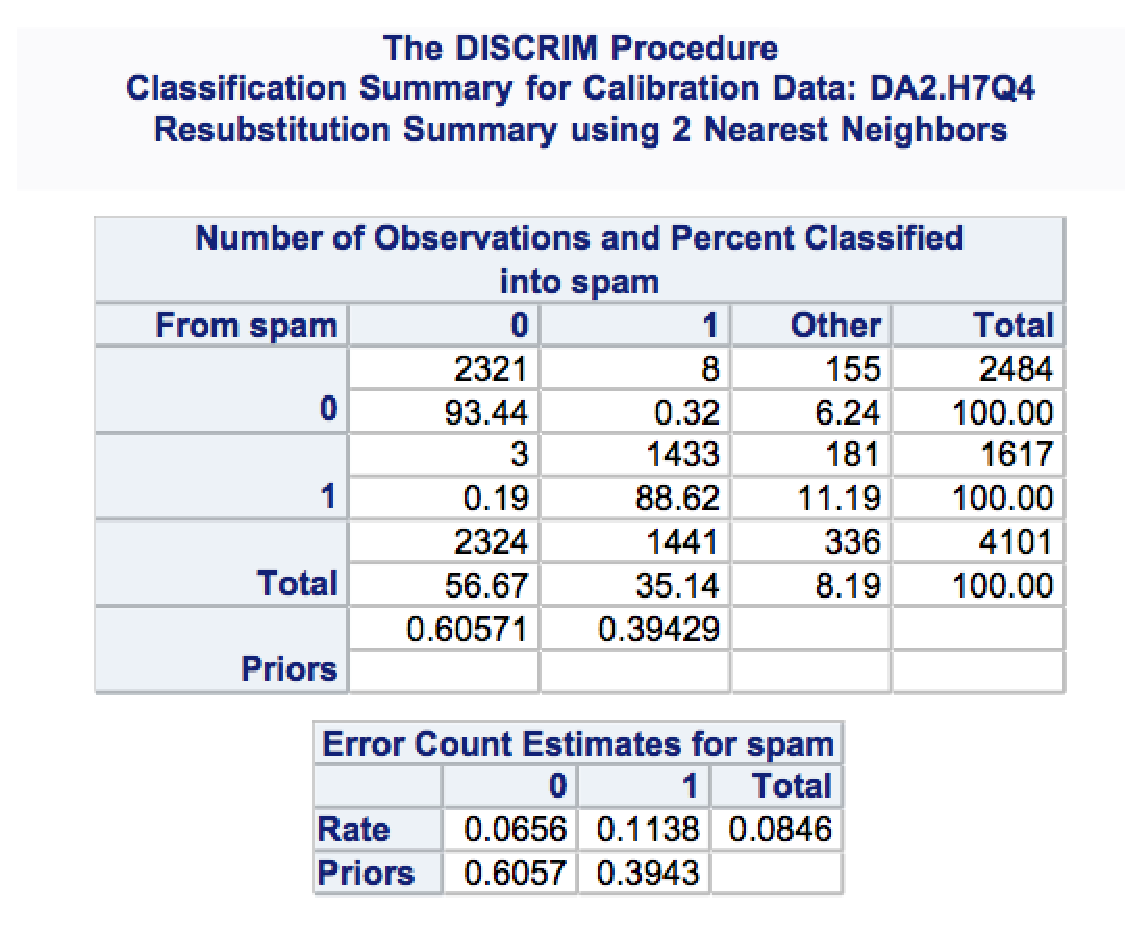
\includegraphics[width=3in]{7-15.eps}
\end{minipage}
\begin{minipage}[t]{0.5\linewidth}
\centering
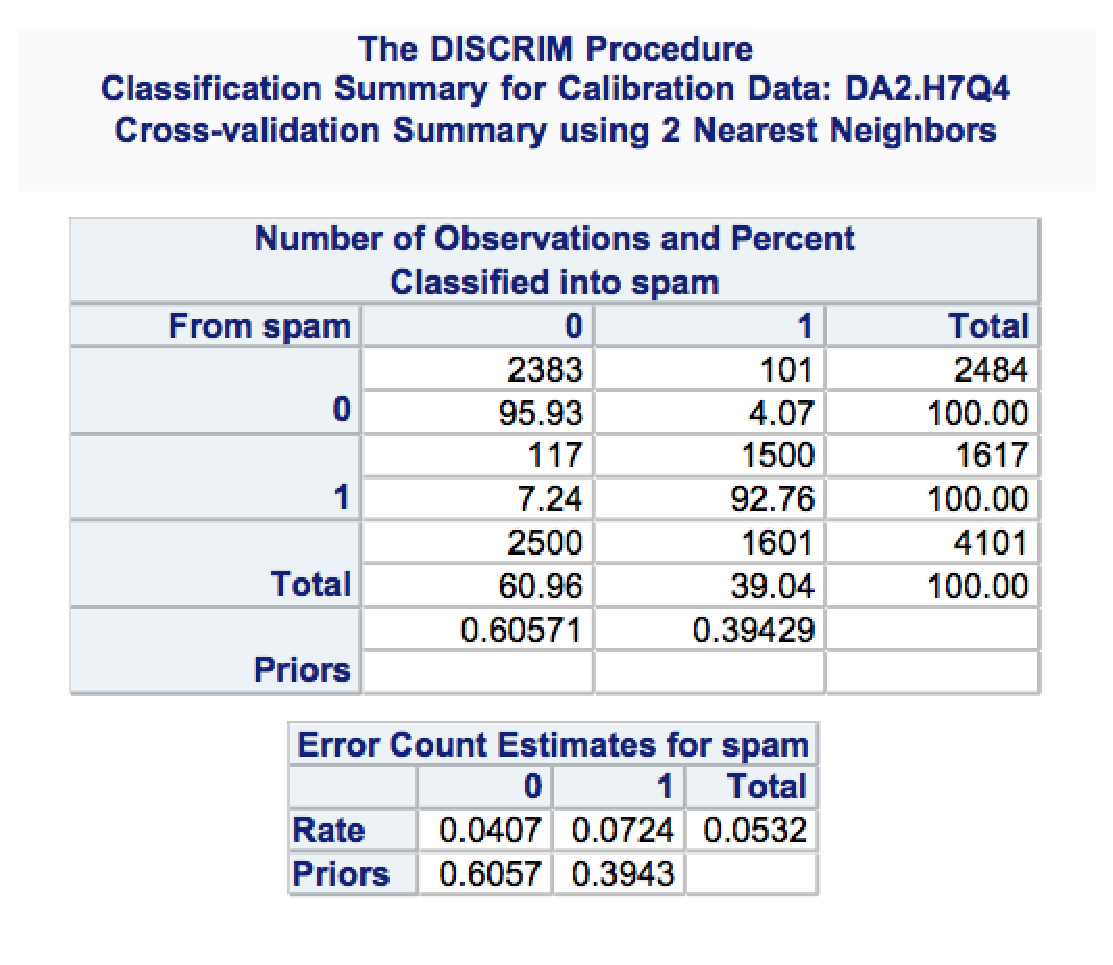
\includegraphics[width=3in]{7-16.eps}
\end{minipage}
\caption{Confusion Table of 2-Nearest Neighbors Classifier}\label{t1}
\end{figure}
\begin{figure}[htbp]
\centering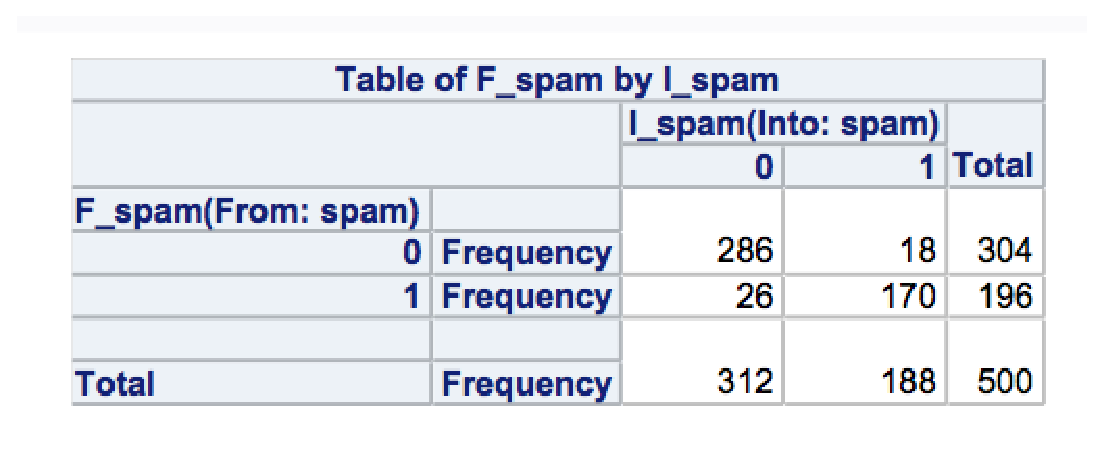
\includegraphics[width=3.5in]{7-25.eps}
\caption{Confusion Table of Logistic Regression}\label{t6}
\end{figure}

\begin{figure}[htbp]
\begin{minipage}[t]{0.5\linewidth}
\centering
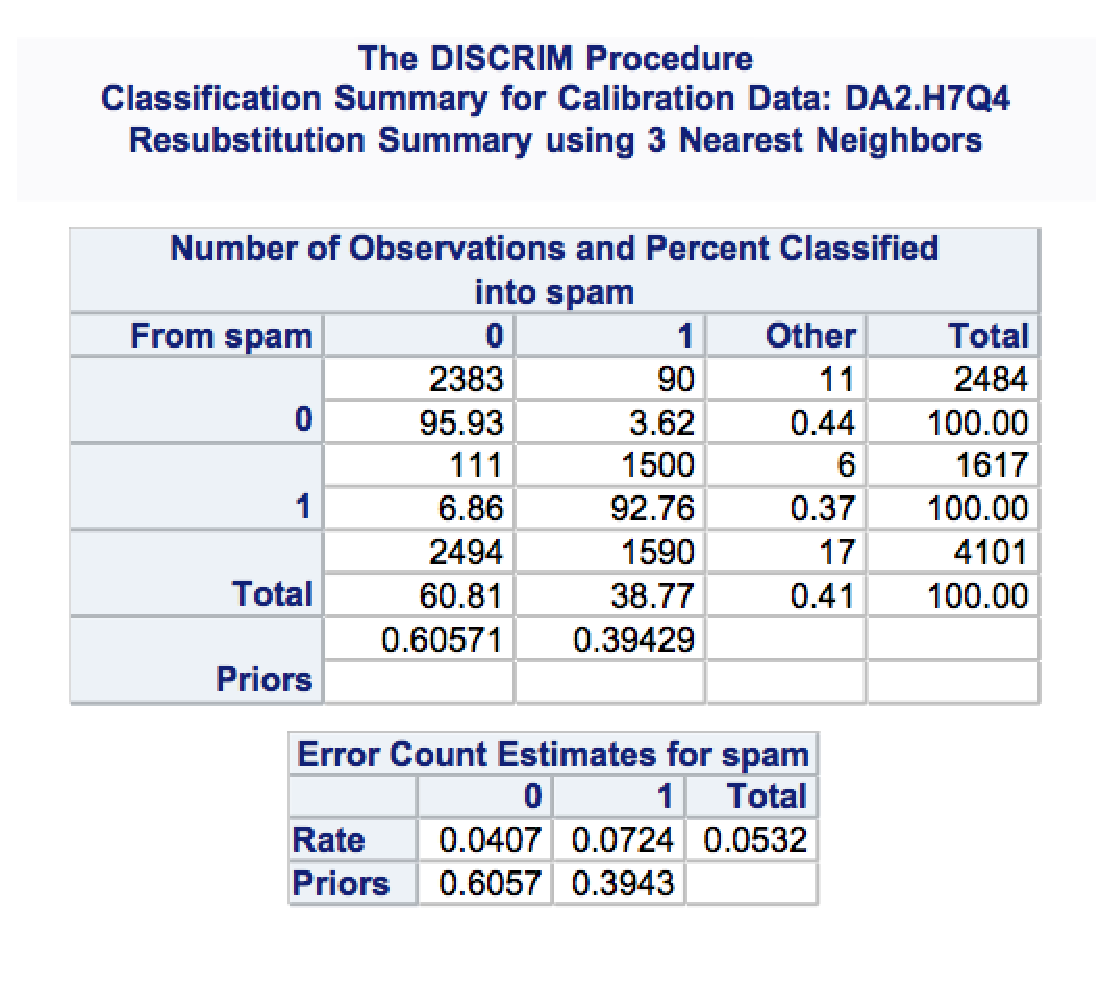
\includegraphics[width=3in]{7-17.eps}
\end{minipage}
\begin{minipage}[t]{0.5\linewidth}
\centering
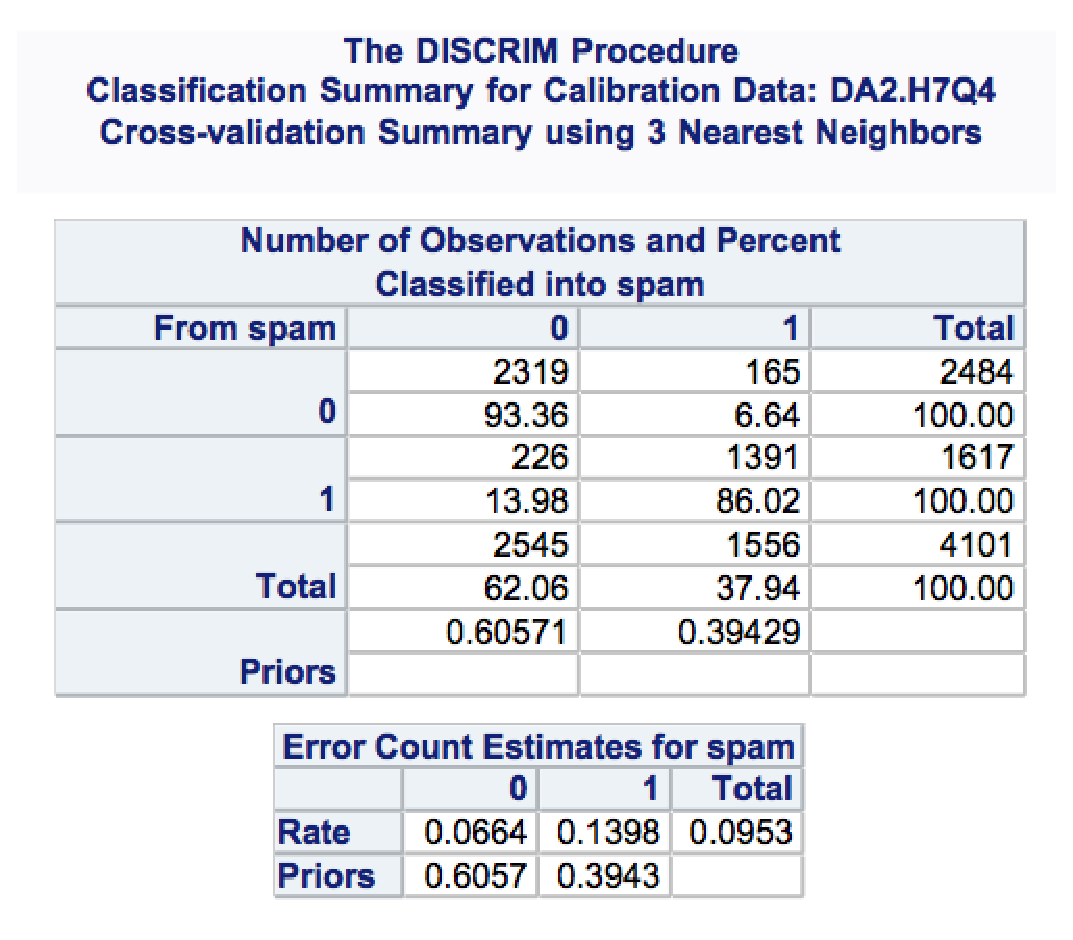
\includegraphics[width=3in]{7-18.eps}
\end{minipage}
\caption{Confusion Table of 3-Nearest Neighbors Classifier}\label{t2}
\end{figure}

\begin{figure}[htbp]
\begin{minipage}[t]{0.5\linewidth}
\centering
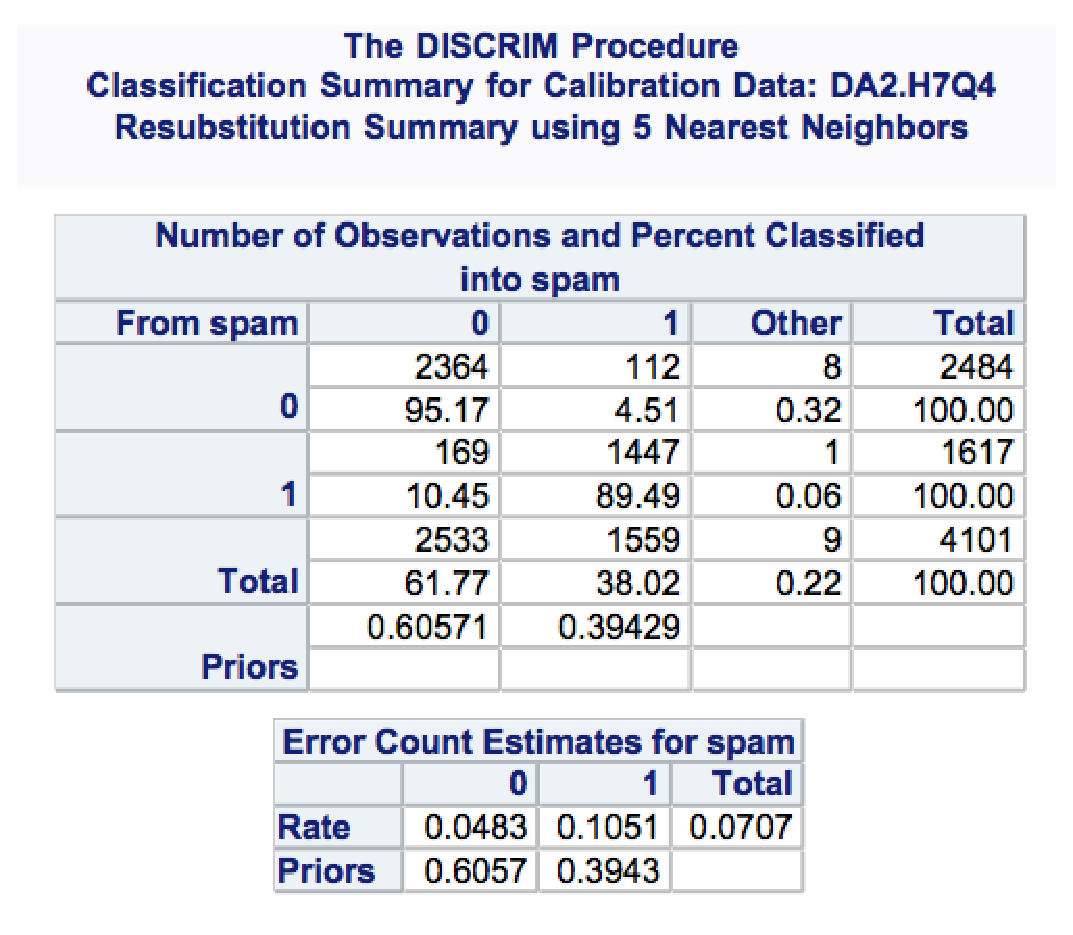
\includegraphics[width=3in]{7-19.eps}
\end{minipage}
\begin{minipage}[t]{0.5\linewidth}
\centering
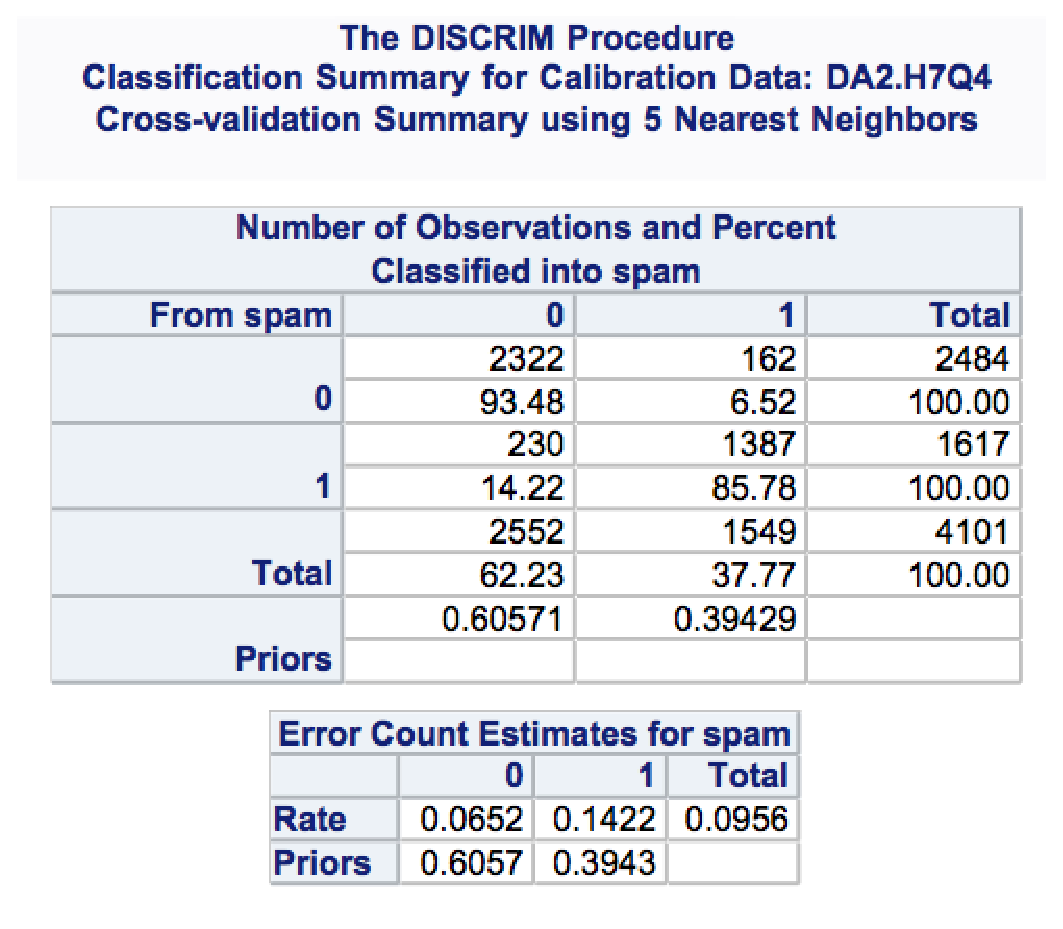
\includegraphics[width=3in]{7-20.eps}
\end{minipage}
\caption{Confusion Table of 5-Nearest Neighbors Classifier}\label{t3}
\end{figure}

\begin{figure}[htbp]
\begin{minipage}[t]{0.5\linewidth}
\centering
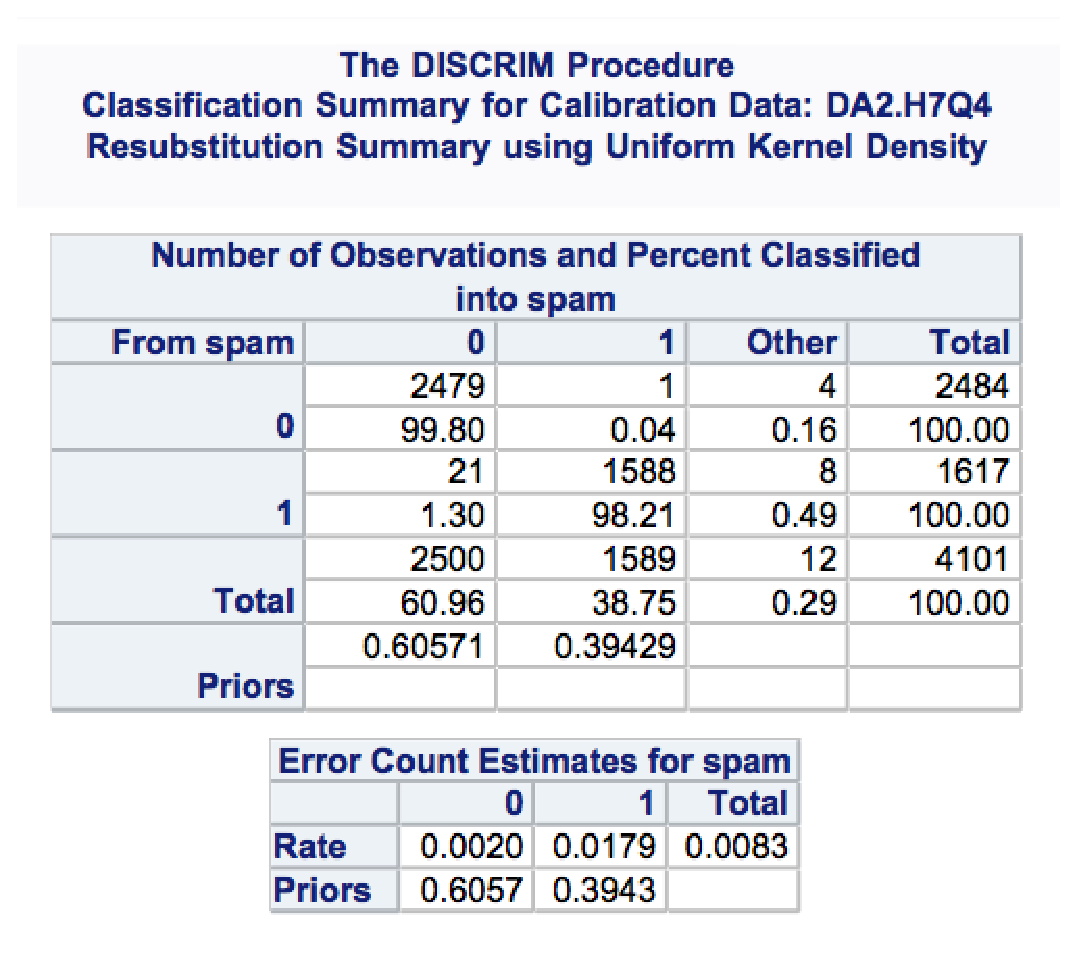
\includegraphics[width=3in]{7-21.eps}
\end{minipage}
\begin{minipage}[t]{0.5\linewidth}
\centering
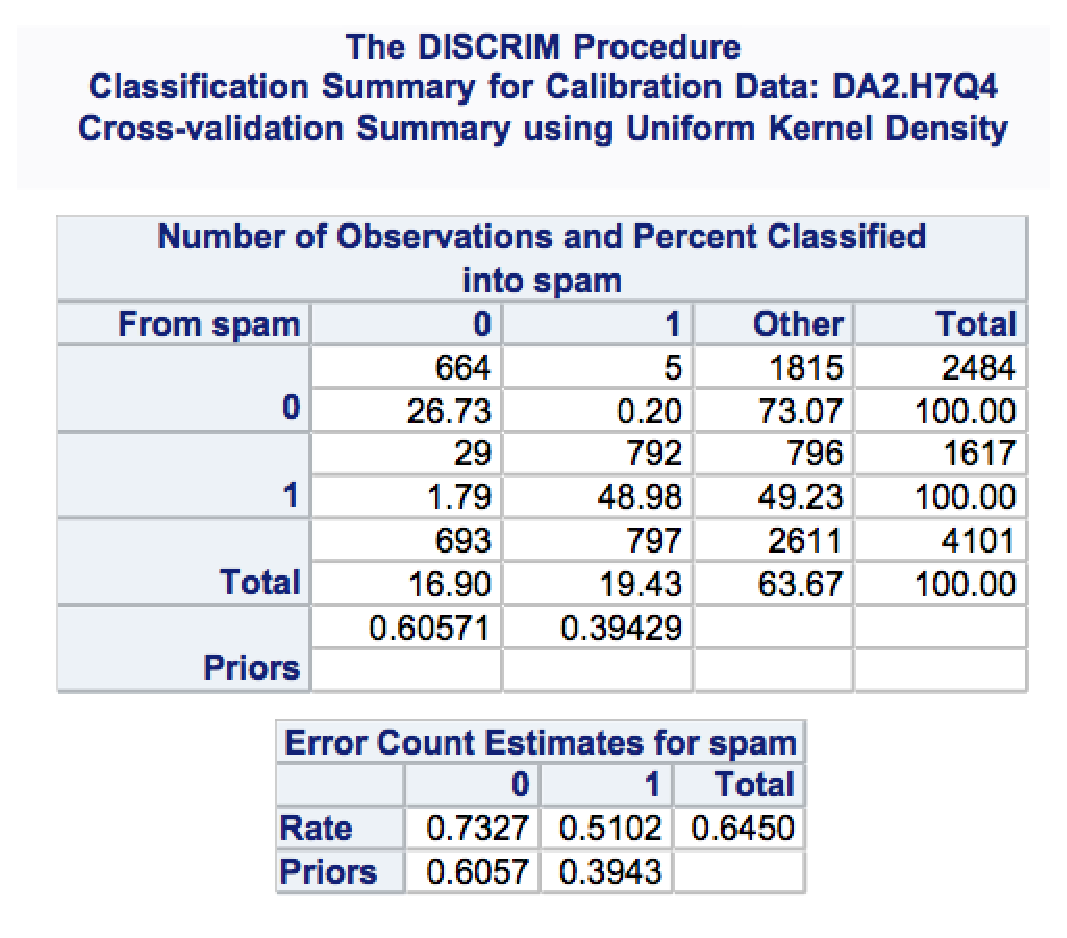
\includegraphics[width=3in]{7-22.eps}
\end{minipage}
\caption{Confusion Table of 1-Radius Kernal Classifier}\label{t4}
\end{figure}

\begin{figure}[htbp]
\begin{minipage}[t]{0.5\linewidth}
\centering
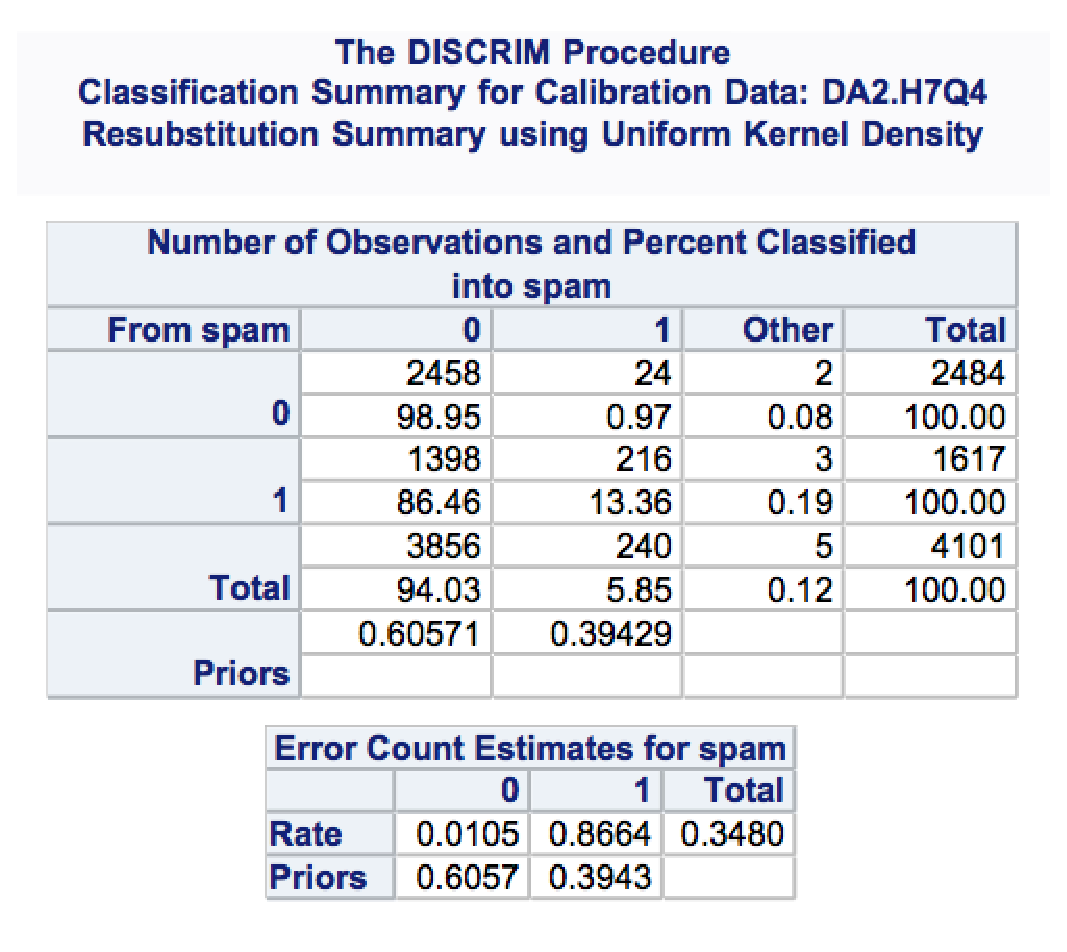
\includegraphics[width=3in]{7-23.eps}
\end{minipage}
\begin{minipage}[t]{0.5\linewidth}
\centering
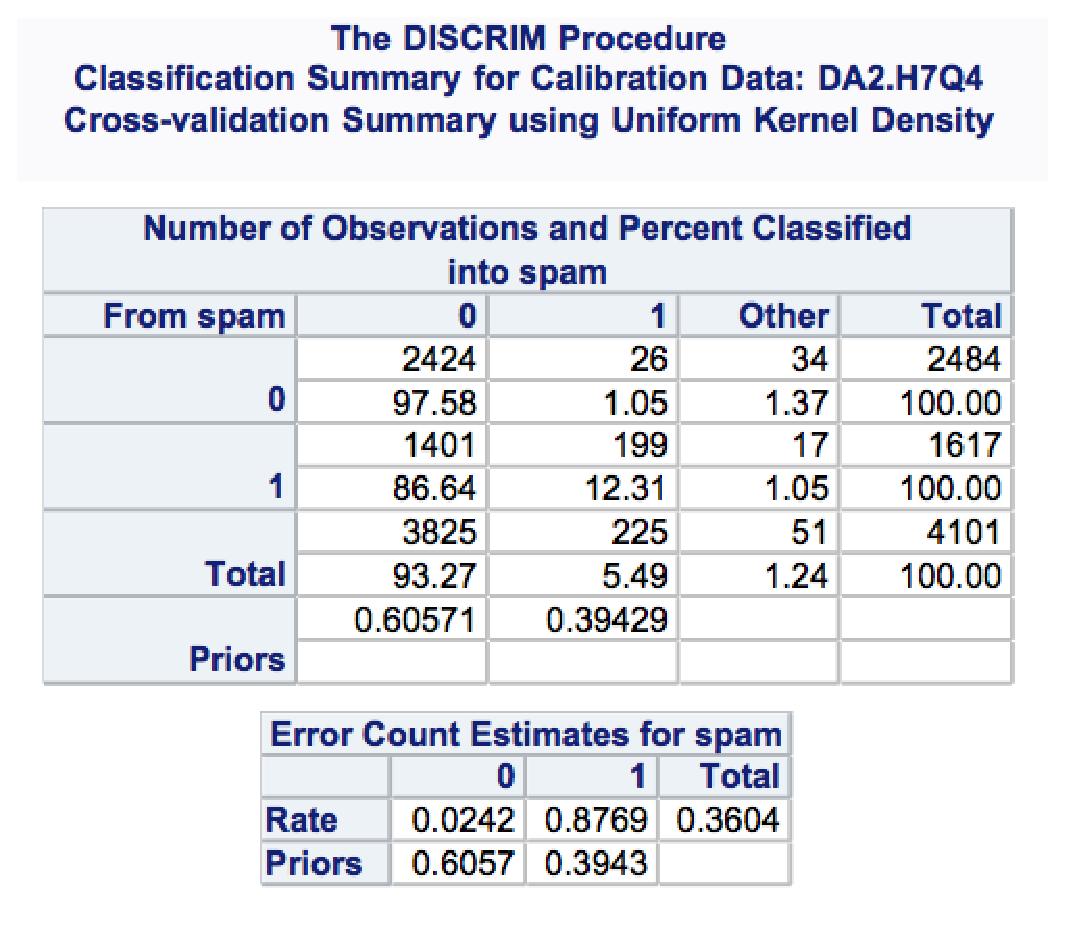
\includegraphics[width=3in]{7-24.eps}
\end{minipage}
\caption{Confusion Table of 10-Radius Kernal Classifier}\label{t5}
\end{figure}












\end{document}
